\documentclass[11pt,spanish]{article}

% Paquetes
\usepackage{amstext}
\usepackage{amssymb}
\usepackage{amsmath}
\usepackage{babel}
    \addto\shorthandsspanish{\spanishdeactivate{~<>}}
    \decimalpoint
\usepackage[style=iso]{datetime2}
\usepackage{fancyhdr}
\usepackage{float}
\usepackage[T1]{fontenc}
\usepackage[a4paper]{geometry}
    \geometry{verbose,tmargin=3cm,bmargin=2cm,lmargin=2.5cm,rmargin=2.5cm}
\usepackage{graphicx}
\usepackage{hyperref}
\usepackage[utf8]{inputenc}
\usepackage{lastpage}
\usepackage{mathptmx}
\usepackage{tasks}
\usepackage{units}
\usepackage{siunitx}

% dibujos 

\usepackage{tikz}
\usepackage{tikz-dimline}
\usetikzlibrary{calc}
% \usetikzlibrary{math}
\usetikzlibrary{arrows.meta}
\usetikzlibrary{snakes}
\usetikzlibrary{decorations}
\usetikzlibrary{decorations.pathmorphing}
\usetikzlibrary{patterns}

% tipo de fuente 
\usepackage{lmodern}

\pagestyle{fancy}
\lfoot{\small DF, FCEyN, UBA}
\cfoot{\tiny Actualizado el {\today} a las {\DTMcurrenttime}}
\rfoot{\small Pág. {\thepage} de \pageref{LastPage}}

\begin{document}

% Título
    \begin{center}
    \textsc{\large Física 2 (Física) -- Cátedra Diego Arbó}
    \par\end{center}{\large \par}
    
    \begin{center}
    \textsc{\large Primer Cuatrimestre de 2025}
    \par\end{center}{\large \par}
    
    \begin{center}
    \textsc{\large Guía 11: Difracción}
    \par\end{center}{\large \par}

% Comienzo 
\begin{enumerate}


\section*{Rendija simple}

% Ejercicio 1

    \item 
    \begin{enumerate}
        \item Considere la figura de difracción de Fraunhofer producida por una
        rendija de ancho $b$ ubicada entre dos lentes convergentes y centrada
        en el eje óptico del sistema. La fuente puntual de longitud de onda
        $\lambda$ se coloca en el foco de la primera lente. a) 
        
        \begin{enumerate}
            \item ¿Dónde se coloca la pantalla de observación?
            \item Calcule la posición de los máximos y de los mínimos de intensidad,
            el ancho angular de la campana principal de difracción y de los máximos
            secundarios. 
            \item Calcule la relación de intensidades entre el máximo principal y el
            primer máximo secundario. 
            \item Grafique la intensidad sobre la pantalla, ¿en función de qué variables
            lo hace?; ¿podría haber elegido otras?, ¿cuáles?
            \item Discuta cómo se modifican los parámetros de la figura de difracción
            si se cambia: 1) el ancho de la ranura, 2) la longitud de onda, 3)
            si se coloca una fuente policromática. 
        \end{enumerate}
        
        \item Idem (a), si la fuente se encuentra en el plano focal de la primera
        lente, a una altura $h$ del eje óptico. 
        
        \item Idem (b), si la ranura se centra a una altura $h'$ del eje óptico. 
    \end{enumerate}

% Ejercicio 2

    \item Una rendija de $50$ $\mu$m de ancho se encuentra entre dos lentes
    delgadas convergentes de igual distancia focal, y está iluminada por
    ondas planas, de longitud de onda $\lambda=5000$ Å. La distancia
    entre el primer mínimo a la izquierda del máximo principal y el tercer
    mínimo a su derecha es de $3$ mm. Además, el primer mínimo a la izquierda
    está ubicado $3$ mm a la derecha del eje óptico.
    
    \begin{enumerate}
        \item ¿Cuál es la distancia focal de las lentes? 
        \item ¿Dónde se encuentra la fuente? ¿Dónde el máximo principal? 
    \end{enumerate}

% Ejercicio 3

    \item Rendija bidimensional:
    
    \begin{enumerate}
        \item Hallar el patrón de intensidades de una abertura rectangular de lados
        $a$ y $b$, que se encuentra a distancia $D$ de una pantalla. Considere
        incidencia normal. 
        
        \item Ídem para una abertura circular de radio $a$.
    \end{enumerate}

% Ejercicio 4

    \item Hallar el campo eléctrico, como función de las coordenadas sobre la
    pantalla, para las configuraciones de la figura, las que se encuentran
    a distancia $D$ de la pantalla. La luz es monocromática de longitud
    de onda $\lambda$ e incide normalmente sobre las aberturas.

    \begin{figure}[H]
        \centering{}
        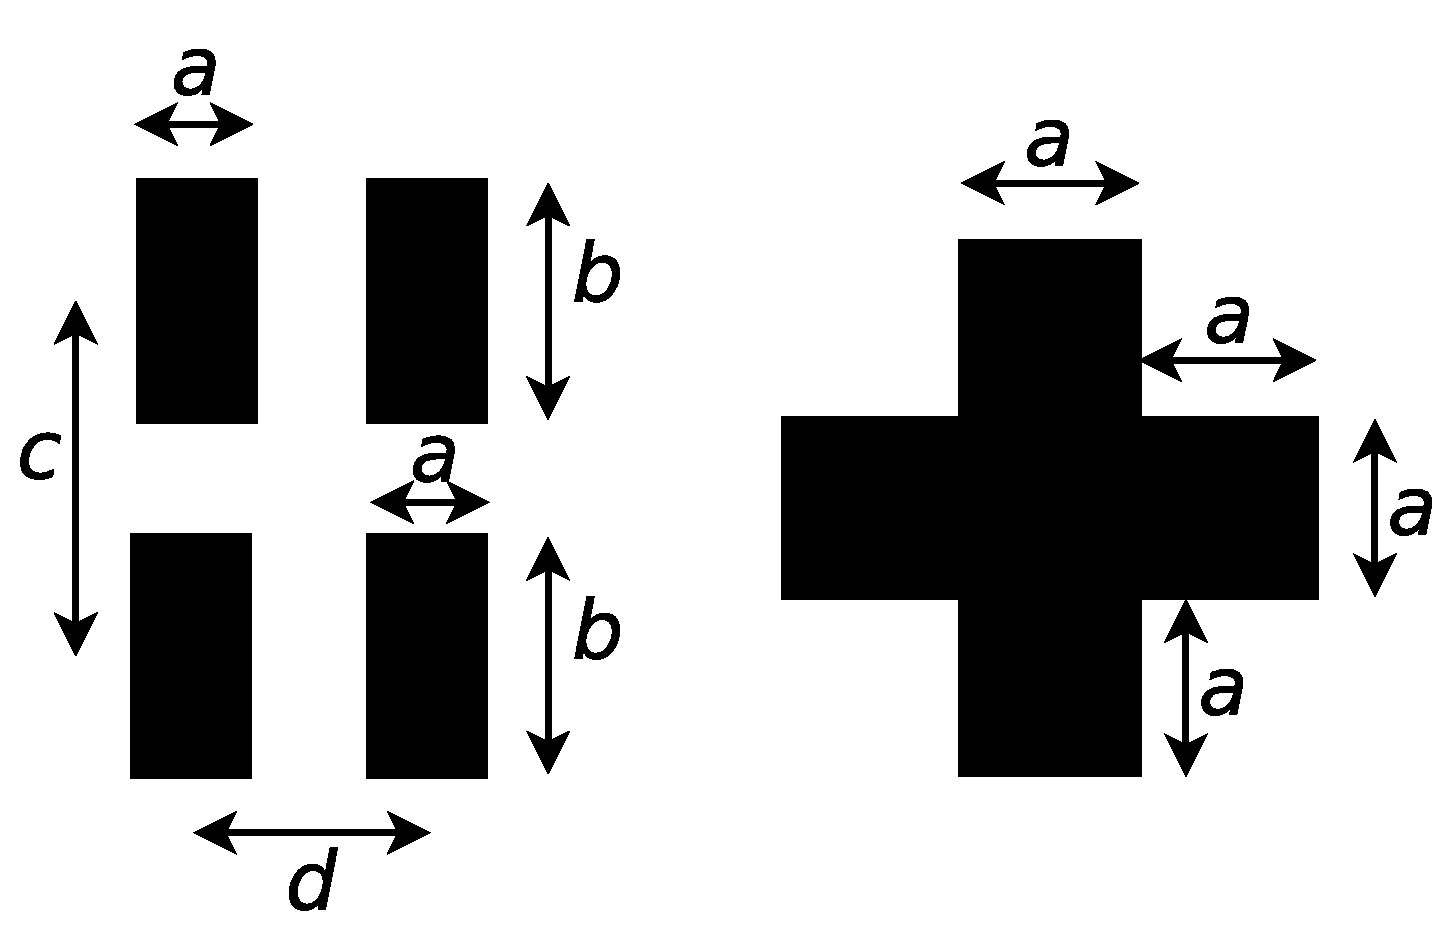
\includegraphics[clip,scale=0.25]{figs/ej5-35}
    \end{figure}


\section*{Doble rendija}

% Ejercicio 5

    \item 

    \begin{enumerate}
        \item Se tienen dos rendijas iguales, de ancho $b$, cuya separación entre
        centros es $d$, colocadas entre dos lentes delgadas convergentes,
        ubicadas en forma simétrica respecto del eje óptico del sistema. Una
        fuente puntual monocromática que emite con $\lambda$ se encuentra
        en el foco de la primera lente. Considere la figura de interferencia--difracción
        de Fraunhofer de la fuente. 
        
        \begin{enumerate}
            \item Calcule la posición de los máximos y mínimos tanto de interferencia
            como de difracción. 

            \item Grafique la intensidad sobre la pantalla, ¿en función de qué variable
            lo hace? ¿Qué otra variable podría haber usado?

            \item Suponiendo que la teoría fuese exacta, ¿qué condiciones deberían cumplirse
            para que desaparezcan órdenes, y cuáles serían los órdenes desaparecidos? 

            \item ¿Cuántos órdenes de interferencia hay dentro de la campana principal
            de difracción?

            \item A la luz de estos resultados discuta el interferómetro de Young. 

            \item Considere que la fuente emite en $\lambda$, $2\lambda$ y $3\lambda$
            simultáneamente. Para cada una de dichas longitudes de onda, ¿cuál
            es la posición de los máximos y mínimos de interferencia y difracción?
            En particular, ¿cuál es la posición del máximo principal?
        \end{enumerate}

        \item Repita lo hecho en (a), si la fuente se encuentra a una altura $h$
        del eje óptico.

        \item Idem (b) si el punto medio entre ranuras se encuentra a una altura
        $h'$ del eje óptico. 
    \end{enumerate}

% Ejercicio 6

    \item Se realiza una experiencia de difracción por doble rendija con una
    fuente que emite en $4000$ Å. La separación entre los puntos medios
    de las rendijas es de $0.4$ mm y el ancho de cada una de ellas es
    de $0.04$ mm. La pantalla está a $1$ m de las rendijas. Luego se cambia
    la fuente por otra que emite en $6000$ Å. Determine:

    \begin{enumerate}
        \item En cuánto varió la interfranja.

        \item En cuánto varió el número total de franjas de interferencia contenidas
        en la campana principal de difracción.

        \item En cuánto varió el ancho angular de la campana principal de difracción.
    \end{enumerate}

% Ejercicio 7
    
    \item Sobre dos ranuras separadas una distancia de $1$ mm incide la superposición
    de dos ondas planas monocromáticas de longitudes de onda $\lambda_{1}$
    y $\lambda_{2}$

    \begin{enumerate}
        \item ¿Qué relación debe satisfacer el cociente $\lambda_{1}/\lambda_{2}$
        para que el tercer orden de interferencia constructiva de $\lambda_{1}$
        coincida con el tercer mínimo de $\lambda_{2}$?

        \item ¿Qué ancho deben tener las ranuras para que además esos órdenes
        coincidan con el primer mínimo de difracción de $\lambda_{1}$? ¿Qué
        intensidad se registrará en la pantalla en ese punto?
    \end{enumerate}


\section*{Redes de difracción y límites de resolución}

% Ejercicio 8

    \item 
    
    \begin{enumerate}
        \item Diga qué entiende por red de transmisión y por red de reflexión.
        Dé ejemplos de cada tipo.

        \item Ídem (a) para red de amplitud y fase. 
    \end{enumerate}

% Ejercicio 9

    \item Una onda plana monocromática de longitud de onda $\lambda$ incide
    normalmente sobre una red de transmisión plana formada por $N$ rendijas
    de ancho $b$ y período $d$ ($b\ll d$). Suponiendo que la teoría
    corresponde a una descripción exacta del fenómeno: 

    \begin{enumerate}
        \item Analice la distribución de intensidad sobre la pantalla y grafíquela.

        \item Calcule la posición angular de las líneas espectrales (¿a qué máximos
        corresponden?), y su intensidad.

        \item Calcule el número de mínimos de interferencia entre dos líneas
        espectrales, por ende, ¿cuántos máximos secundarios hay?

        \item Calcule el ancho angular de las líneas espectrales.

        \item Calcule el máximo orden observable.

        \item Discuta: 
        
        \begin{enumerate}
            \item ¿Qué aproximación hace en los ángulos?

            \item La dependencia de los parámetros con el número de rendijas y
            con la densidad de rendijas.
        \end{enumerate}
    \end{enumerate}

% Ejercicio 10

    \item Sobre la red del problema anterior incide la superposición de dos
    ondas planas monocromáticas de longitudes de onda $\lambda$ y
    $\lambda+\Delta\lambda$, calcule: 

    \begin{enumerate}
        \item La dispersión angular.

        \item El poder resolvente.

        \item El máximo poder resolvente.

        \item Grafique la intensidad sobre la pantalla.

        \item Recalcule el problema anterior para una incidencia distinta de la
        normal, y discuta si existe alguna ventaja al trabajar de esa manera.
    \end{enumerate}

% Ejercicio 11
    
    \item Se dispone de dos redes de difracción cuadradas de $2$ cm de lado; una
    tiene $600$ líneas/mm y la otra $1200$ líneas/mm. Calcule:

    \begin{enumerate}
        \item El poder resolvente de cada red en el primer orden.

        \item Si la fuente emite en $5000$ Å, el máximo orden observable. ¿Es 
        importante tener en cuenta el ángulo de incidencia?
        
        \item El máximo poder resolvente de cada una.
        
        \item Si alguna de ellas resuelve las siguientes longitudes de onda: 
        $\lambda_{1}=5000$ Å y $\lambda_{2}=5000.07$ Å.
        
    \end{enumerate}

% Ejercicio 12

    \item Se tiene un dispositivo como el que se muestra en la figura, formado
    por una red dispuesta entre dos lentes. La red es iluminada por dos
    fuentes $S_{1}$ y $S_{2}$ que emiten luz con la misma intensidad,
    pero con longitudes de onda $\lambda_{1}$ y $\lambda_{2}$ respectivamente.
    Se sabe que la red es de rendijas, pero no se conocen sus parámetros
    ($N$: número de rendijas; $b$: ancho de cada rendija; $d$: período
    de la red). Para poder caracterizarla, se realizan observaciones de
    la figura de difracción--interferencia producida en el plano de observación.
    A partir de lo cual se logra determinar que:

    \begin{itemize}
        \item El orden $-1$ de interferencia correspondiente a $\lambda_{2}$ se
        encuentra una distancia $a_{0}$ por encima del orden $+1$ correspondiente
        a $\lambda_{1}$. 
        
        \item El ancho de la campana de difracción correspondiente a $\lambda_{1}$
        es $d_{0}$.
    \end{itemize}
    
    \begin{figure}[H]
        \centering{}
        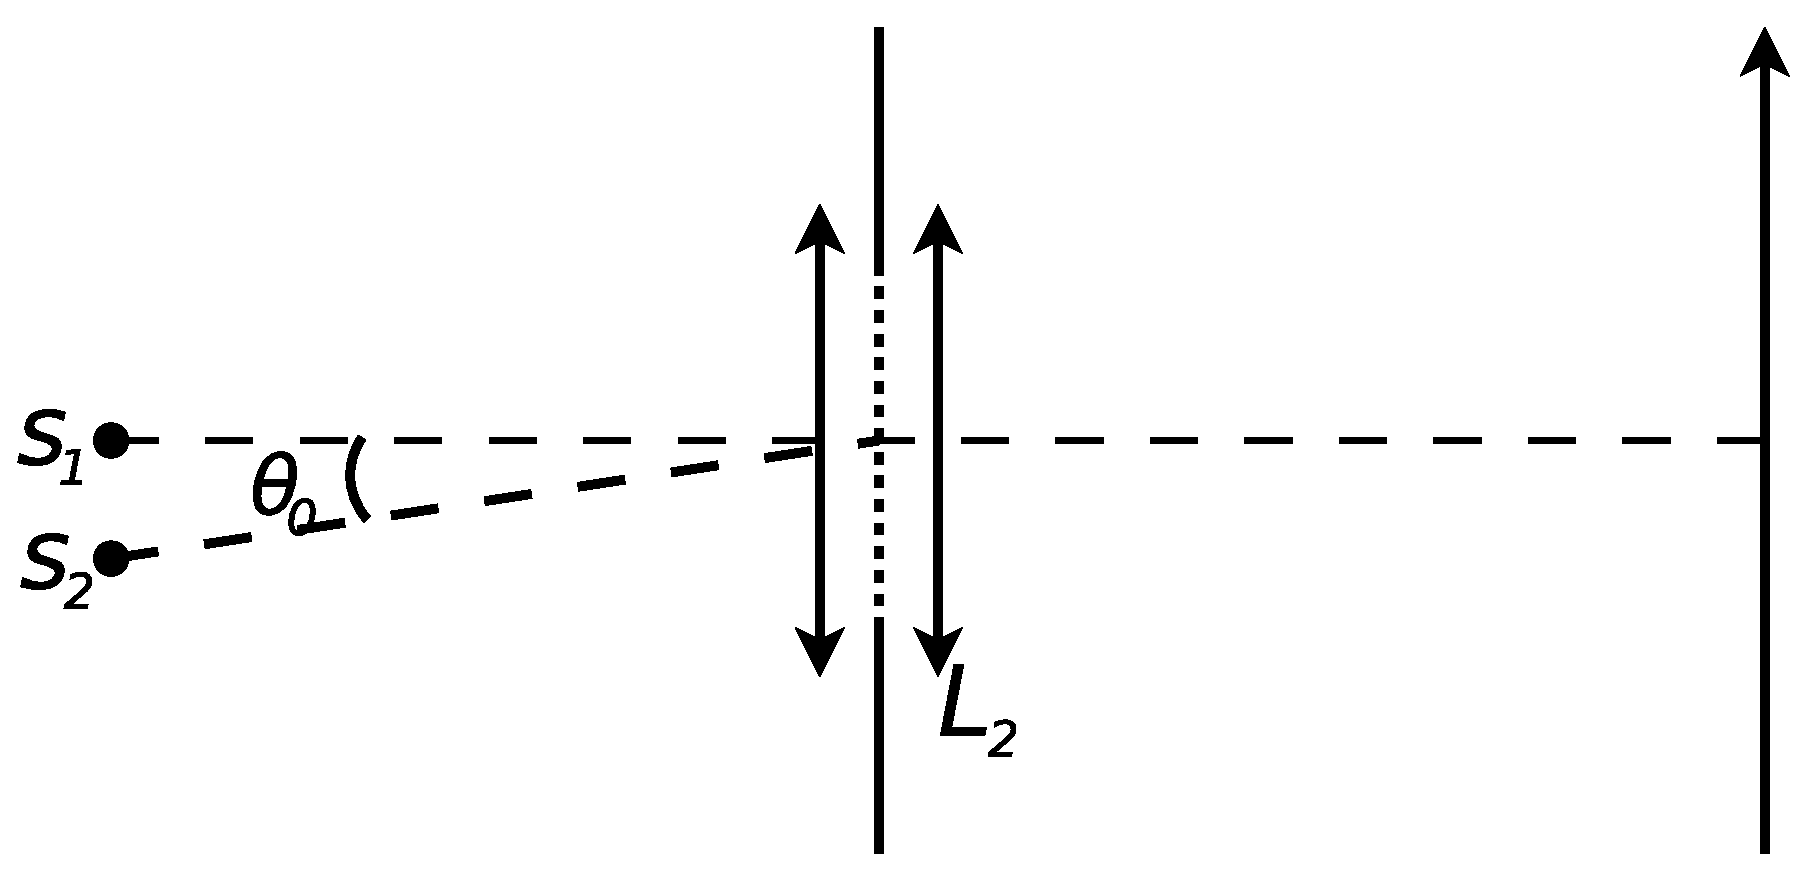
\includegraphics[clip,scale=0.3]{figs/ej5-43}
    \end{figure}
    
    \begin{description}
        \item [{Datos:}] $\sin(\theta_{0})=0.01$; distancia focal de la lente
        $L_{2}=3$ m; $\lambda_{1}=4000$ Å y $\lambda_{2}=5000$ Å; $a_{0}=0.1$
        mm; $d_{0}=10$ cm.
    \end{description}
    
    \begin{enumerate}
        \item Dar la expresión para la distribución de intensidad que se observa
        en la pantalla y justificar por qué la escribe así. Hacer un gráfico
        muy cualitativo de dicha distribución (que dé una idea básica de lo
        que se va a observar).

        \item Determinar las posiciones angulares de todos los ceros de 
        interferencia y difracción.

        \item Determinar las posiciones de los órdenes de interferencia.

        \item Encontrar los parámetros de la red $b$ y $d$.

        \item Ambos órdenes (¡cuidado; se trata de órdenes diferentes!) están
        suficientemente separados entre sí, según el criterio de Rayleigh.
        Hallar una cota para $N$.
    \end{enumerate}

% Ejercicio 13

    \item 

    \begin{enumerate}
        \item Escriba la función transmisión para una red de rendijas de ancho 
        $b$ y período $d$.

        \item Idem (a) para una red formada por prismas delgados de alto $b$ y
        base $a$, con índice de refracción $n$, y separados por tramos obstruidos
        de alto $d-b$ (ver figura).
    \end{enumerate}
    
    \begin{figure}[H]
        \centering{}
        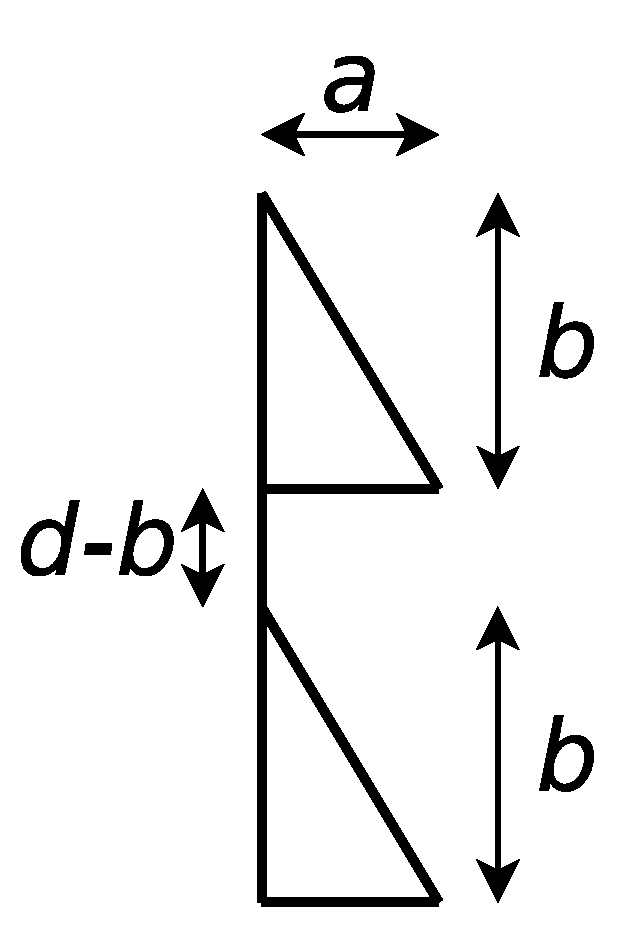
\includegraphics[clip,scale=0.3]{figs/ej5-44}
    \end{figure}

% Ejercicio 14
    \item 
    
    \begin{enumerate}
        \item Hallar la distribución de intensidades sobre la pantalla para la red
        de transmisión descripta en el problema 13b. La luz incide con un
        ángulo arbitrario sobre la red.

        \item Comparar la distribución obtenida con la de una red de transmisión
        de $N$ rendijas de ancho $b$ y período $d$. ¿En qué se diferencian? 
    \end{enumerate}

% Ejercicio 15

    \item Se tiene una red de difracción de $N$ períodos como se muestra en
    la figura. Se trata de una distribución de pares de prismas delgados
    de índices $n_{1}$, y $n_{2}$ y ángulos $\delta_{1}$ y $\delta_{2}$,
    respectivamente (ver figura). Se la ilumina en forma normal. Suponiendo
    que la teoría fuese exacta:

    \begin{figure}[H]
        \centering{}
        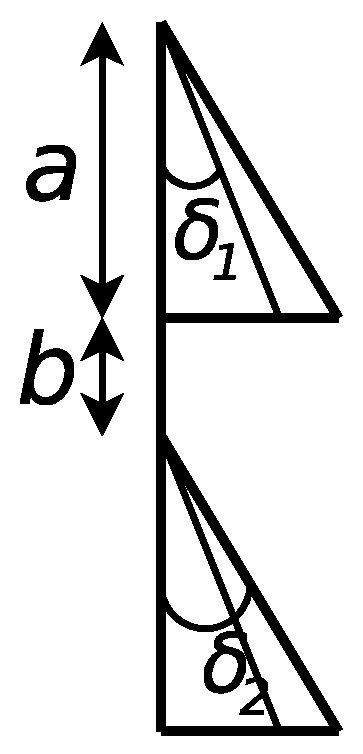
\includegraphics[clip,scale=0.3]{figs/ej5-46}
    \end{figure}

    \begin{enumerate}
        \item Halle la intensidad en la pantalla como función del ángulo $\theta$. 
        \item Elija parámetros de la red ($n_{1}$, $n_{2}$, $\delta_{1}$, $\delta_{2}$,
        $a$, $b$, $N$), para los cuales se intensifique el orden ($-2$)
        para una longitud de onda incidente de $5000$ Å, y para que se puedan
        resolver las longitudes de onda de $5000$ Å y $5001$ Å, en dicho orden.
    \end{enumerate}

% Ejercicio 16

    \item Una red de transmisión de ancho $2$ cm está formada por $50$ prismas
    delgados. Sabiendo que intensifica el segundo orden de interferencia, para
    $\lambda=5000$ Å calcule: 

    \begin{enumerate}
        \item El ángulo de \textit{blaze}.

        \item La posición angular del orden intensificado y de la imagen geométrica.

        \item Discuta, en este caso, qué sucede con los otros órdenes de interferencia
        para la longitud de onda $\lambda$ dada.

        \item Calcule el poder resolvente para el segundo orden. 
    \end{enumerate}

% Ejercicio 17
    
    \item Se desea estudiar la estructura de una banda en la proximidad de $4300$
    Å, utilizando una red plana de reflexión de $10$ cm y $1200$ líneas/mm.
    Hallar:
    
    \begin{enumerate}
        \item El máximo orden observable.

        \item El mínimo ángulo de incidencia para el cual se observa.

        \item El mínimo intervalo de longitudes de onda resueltas.

        \item El orden intensificado. ¿Es ventajoso? Justifique su respuesta.
    \end{enumerate}

% Ejercicio 18

    \item Una red de fase por reflexión tiene $4800$ facetas/cm y ha sido construida
    para intensificar el primer orden, en $\lambda=0.6$ $\mu$m. 

    \begin{enumerate}
        \item Hallar el ángulo que forman las caras facetadas con el plano de la
        red.

        \item Suponiendo incidencia normal, calcular la dispersión angular para
        esa $\lambda$.

        \item Si se iluminase la red con $\lambda=0.48$ $\mu$m, ¿qué órdenes se
        verían?
    \end{enumerate}

% Ejercicio 19

    \item Sean dos fuentes puntuales incoherentes colocadas en el plano focal
    objeto de una lente convergente; ambas emiten la misma $\lambda$.
    A la derecha de la lente hay una ranura de ancho $b$, y luego una
    segunda lente. Se observa la figura de difracción de Fraunhofer de
    las fuentes.

    \begin{enumerate}
        \item Calcule la mínima separación angular entre las fuentes, y la correspondiente
        mínima separación lineal, para que las imágenes estén justamente resueltas
        según el criterio de Rayleigh. Discuta los casos en que ambas fuentes
        emiten con la misma intensidad, y en que no.

        \item Repita el cálculo efectuado en (a) si la rendija se reemplaza por
        una abertura circular de diámetro $d$.
    \end{enumerate}

% Ejercicio 20

    \item Suponga al ojo humano limitado por difracción, y calcule el mínimo
    ángulo que resuelve para un diámetro de pupila de $2$ mm. Si dos puntos
    se hallan a la distancia de visión clara ($25$ cm), ¿cuál es la mínima distancia
    entre ellos para que estén justamente resueltos?

% Ejercicio 21
    
    \item Repita el ítem anterior para un diámetro de pupila de $8$ mm
    (condición de muy poca luz).

\end{enumerate}

\end{document}
